\documentclass[12pt, a4paper, twoside]{article}
\usepackage{tikz}
\usetikzlibrary{calc}
\usepackage{graphicx}
\usepackage{amsmath}
\usepackage[margin=0.8in]{geometry}
\usepackage{listings}
\usepackage{float}
\usepackage{fancyhdr}
\usepackage{indentfirst}
\usepackage[inline]{enumitem}
\usepackage{tabularx}
\usepackage{xcolor}
\usepackage{array}
\usepackage{minted}
\usemintedstyle{vs}
\usepackage[belowskip=0pt,aboveskip=0pt,font=small,labelfont=small]{caption}
\captionsetup{width=\linewidth}

\makeatletter
\newcommand*\circled[1]{\tikz[baseline=(char.base)]{
    \node[shape=circle, draw, inner sep=1pt, 
        minimum height={\f@size*1.25},] (char) {\vphantom{WAH1g}#1};}}
\makeatother

\def \courseNumber {EE2703}
\def \assignmentNumber {10}
\def \myName {Akilesh Kannan}
\def \rollNumber {EE18B122}

\setlength\intextsep{0pt}
\graphicspath{{plots/}}
\setlist[itemize]{noitemsep, topsep=0pt}
\fancyhead[RO,LE]{\courseNumber : Assignment \assignmentNumber}
\fancyhead[LO,RE]{\myName}
\cfoot{\thepage}

\title{\courseNumber : Assignment \assignmentNumber}
\author{\myName\ (\rollNumber)}
\date{\today}

\pagestyle{fancy}

\begin{document}
\maketitle

\section{Introduction}
In this assignment, we shall explore the convolution of two discrete-time signals. We shall look at \textit{linear convolution} and \textit{circular convolution} and their relationship. We shall also look at a certain sequence called \textit{Zadoff-Chu sequence}, and it's special properties.

\section{The FIR Filter}
The given FIR Filter is this:
\begin{figure}[H]
    \centering
    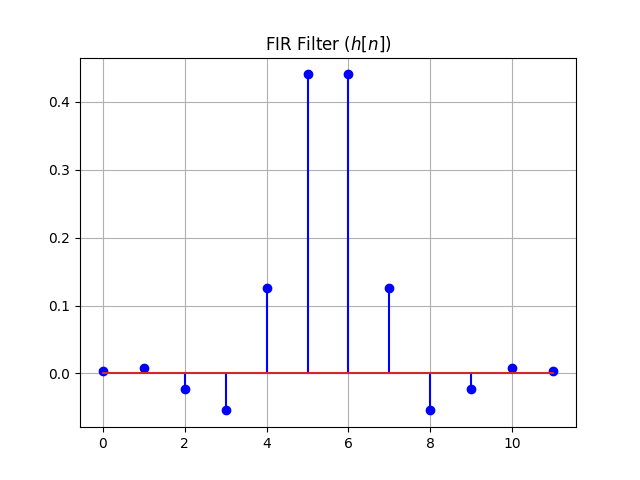
\includegraphics[scale=0.5]{Fig0.png}
    \caption{FIR Filter $h[.]$}
    \label{fig:Fig0}
\end{figure}
If we observe carefully, we can see that the envelope of the filter looks like a $sinc(x)$ function, which means that it's DTFT will look similar to a $rect(\omega)$. 

The magnitude and phase response of the given filter is given by:
\begin{equation}
    H(e^{j\omega}) = \sum_{n=0}^{11}h[n]e^{-j\omega n}
\end{equation}
Using the command \texttt{scipy.signal.freqz}, we shall be able to get the frequency response as shown below:
\begin{figure}[H]
    \centering
    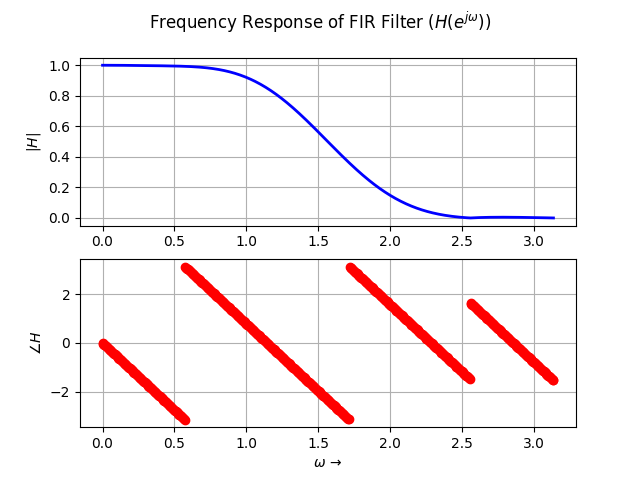
\includegraphics[scale=0.5]{Fig1.png}
    \caption{Frequency Response of FIR Filter $H(e^{j\omega})$}
    \label{fig:Fig1}
\end{figure}

Since, the sequence $h[.]$ is real, it's DTFT $H(e^{j\omega})$ will be even\footnotemark. So, we can see that the magnitude response indeed looks like similar to $rect(\omega)$. \footnotetext{$H(e^{-j\omega}) = \sum_{n=0}^{11}h[n]e^{j\omega n} = H^*(e^{j\omega})\ \implies\ |H(e^{-j\omega})| = |H(e^{j\omega})|$}
\section{Linear Convolution}
Now, we shall take an input signal $x[n] = cos(0.2\pi n)+cos(0.85\pi n)$, and observe the output of the filter.
\begin{figure}[H]
    \centering
    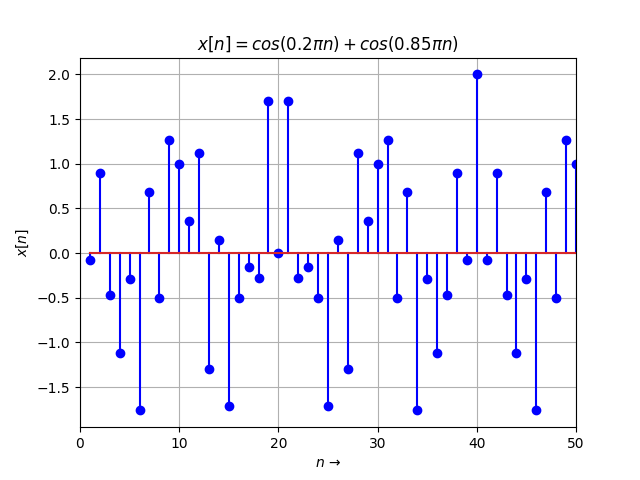
\includegraphics[scale=0.5]{Fig2.png}
    \caption{Input to filter, $x[.]$}
    \label{fig:Fig2}
\end{figure}

The output of the filter $y[.]$ can be got by linear convolution of the input $x[.]$ and the filter's impulse response $h[.]$
\begin{equation}
    y[n] = x\ast h = \sum_{\{k:\ h[k]\neq 0\}}x[n-k]h[k]
\end{equation}

Using the command \texttt{numpy.convolve} to perform the linear convolution operation of $x[.]$ and $h[.]$, we get:
\begin{figure}[H]
    \centering
    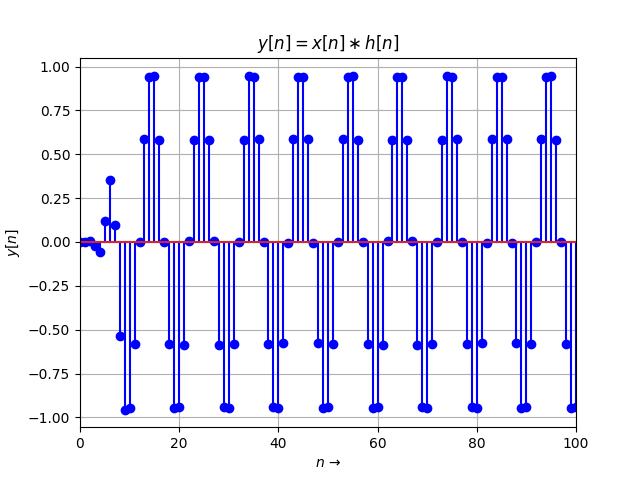
\includegraphics[scale=0.5]{Fig3.png}
    \caption{Output of Filter, $y[n]$}
    \label{fig:Fig3}
\end{figure}

As expected, we see a sinusoid of frequency approximately $0.2\pi$. This is because the filter has damped the high frequency component $cos(0.85\pi n)$ greatly. We can see from the magnitude response that $|H(e^{j\omega})| \Big{\lvert}_{\omega=0.85\pi}$ is close to 0.

\section{Circular Convolution}
An N-point circular convolution is defined as:
\begin{gather}
    y[.] = x[.]\ \text{\circled{N}}\ h[.]\\
    y[n] = \sum_{m=0}^{N-1}x[m]h[(n-m)\mod N],\ n\in [0, N-1]
\end{gather}

Here, the length of all the three signals involved, $x[.]$, $h[.]$ and $y[.]$ are the same and equal to $N$.

We can easily see that the $y[.]$ obtained as a result of circular convolution and that obtained by linear convolution will not be same always. However, if we take an P-point circular convolution, by appropriately zero padding the two signals, such that $P \geq len(y_{lin}[.])$, then, the two will match. This is because $y_{cir}[.]$ is the principal period of $\tilde{y}_{lin}[.]$, which is a periodic extension of $y_{lin}[.]$, with period $P$. So, if the period $P < len(y_{lin}[.])$, then there will be time-aliasing, which will distort the output. Otherwise, if $P \geq len(y_{lin}[.])$, then, there will not be any time-aliasing and so, $y_{cir}[.]$ and $y_{lin}[.]$ will have the same information.

We get the following graphs, depending on the length of the circular convolution output.

\begin{enumerate}[label= \texttt{Case (\alph*)}]
    \item $N = 1024$
    \begin{figure}[H]
        \centering
        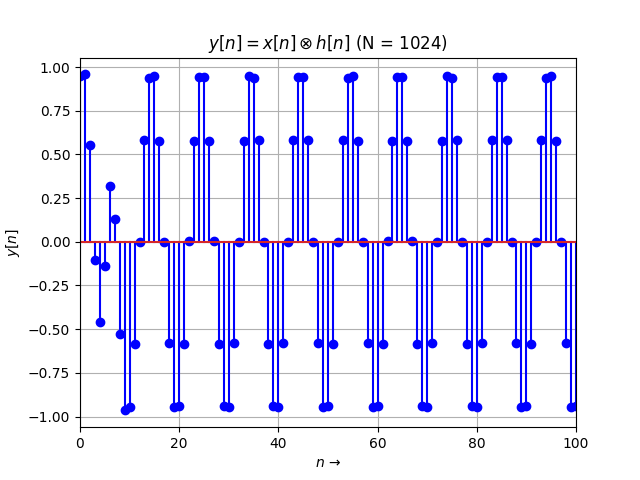
\includegraphics[scale=0.5]{Fig4.png}
        \caption{1024-point circular convolution}
        \label{fig:Fig4}
    \end{figure}
    \item $N = 1034$
    \begin{figure}[H]
        \centering
        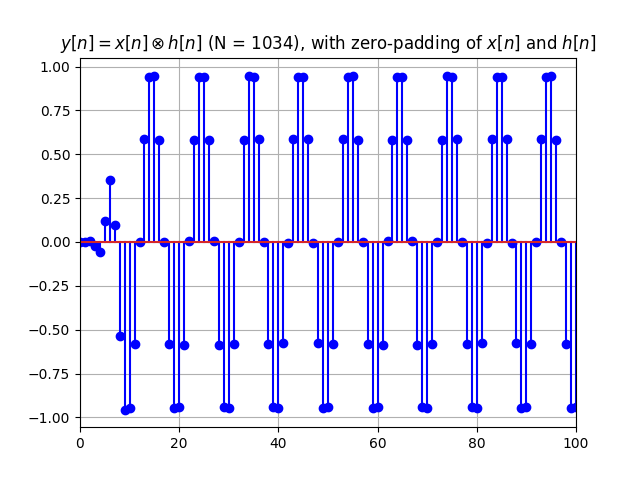
\includegraphics[scale=0.5]{Fig5.png}
        \caption{1034-point circular convolution}
        \label{fig:Fig4}
    \end{figure}
\end{enumerate}

Here, we can see that the 1034-point circular convolution results in the same output as linear convolution. This is because, the length of linear convolution signal is $1024 + 11 - 1 = 1034$. Thus, we have implemented linear convolution using circular convolution.

But, to efficiently implement linear convolution through circular convolution, we have to take $2^m$-point circular convolution. This is because, the underlying algorithm, the \textit{Fast Fourier Transform} (FFT) is most efficient when it is used for $2^m$-point signals.

\section{Circular Correlation of Zadoff-Chu Sequence}
Consider the Zadoff-Chu sequence, a commonly used sequence in communication. The properties of the sequence are:
\begin{enumerate}
    \item It is a complex sequence.
    \item It is a constant amplitude sequence.
    \item The auto correlation of a Zadoff-Chu sequence with a cyclically shifted version of itself is zero, except at the shift.
    \item Correlation of Zadoff-Chu sequence with a delayed version of itself will give a peak at that delay.
\end{enumerate}

The Zadoff-Chu sequence is shown below:
\begin{figure}[H]
    \centering
    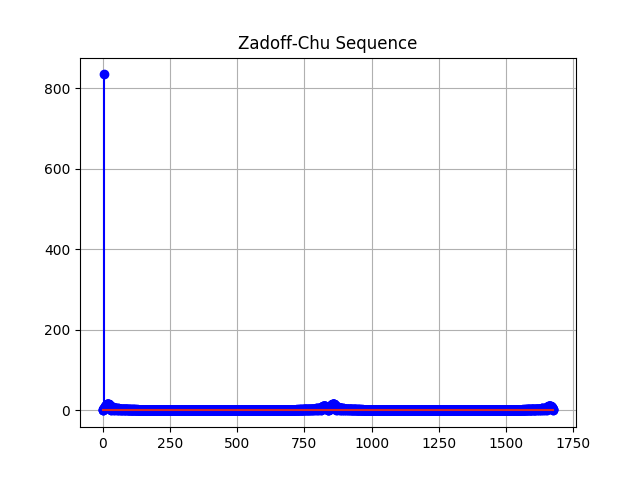
\includegraphics[scale=0.5]{Fig6.png}
    \caption{Zadoff-Chu Sequence}
    \label{fig:Fig6}
\end{figure}

We can verify property (3) given above, by plotting the auto-correlation of $zChu[.]$ with a cyclically delayed version of itself. I have taken the auto-correlation with $zChu[.]$ cyclically rotated by 5. The result was:
\begin{figure}[H]
    \centering
    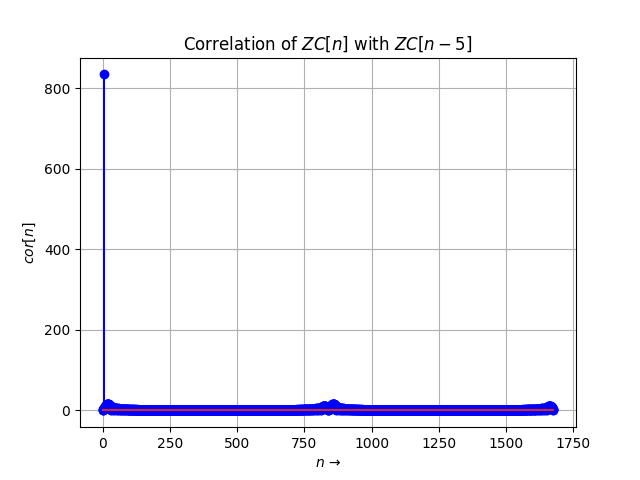
\includegraphics[scale=0.5]{Fig7.png}
    \label{fig:Fig7}
\end{figure}
\begin{figure}[H]
    \centering
    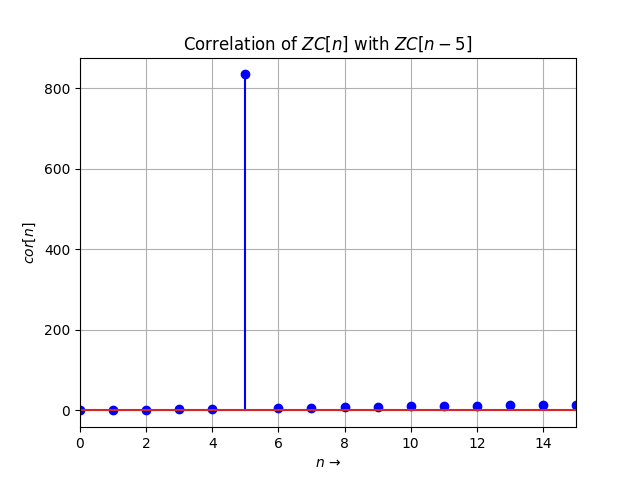
\includegraphics[scale=0.5]{Fig8.png}
    \caption{Auto-correlation of $zChu[.]$ with a cyclically delayed version of itself}
    \label{fig:Fig7}
\end{figure}
In the above figure, we can see that the auto-correlation is non-zero only at $n=5$, which corresponds to the delay value.

\section{Conclusion}
Linear convolution algorithm implemented using a direct summation is non-optimal and computationally expensive.  A faster way to perform the convolution is to use the DFTs of the input and the filter.  Circular convolution can be used for the implementation of linear convolution, with a much faster computation speed.  The magnitude and phase response of a low pass filter were studied and the system’s output, for a mixed frequency signal was obtained through three different methods.  For the Zadoff-Chu sequence, it's auto-correlation with a cyclically shifted version of itself was found to be non-zero only at the point corresponding to the shift.
\end{document}
